\documentclass[a4paper]{scrartcl}

% UTF-8 encoding
\usepackage[utf8]{inputenc}

% include 
\usepackage{graphicx}

% Meta informations
\title{1 PatchMatch Algorithm}
\subtitle{Computer Vision 2 \\ TU Dresden}
\author{Lucas Kahlert}
\date{\today}

\begin{document}

\maketitle


\section{Visualization}

Like in the Computer vision practical seminar in the winter semester 2014 I use
Gunnar Farneback's algorithm to calculate a dense optical flow. The script is
called \texttt{visual.py}. The intensity is reversed compared to the Middlebury
benchmark visualization. Black means no movement instead of white.

You could apply a different normalization method. In the current approach we
normalize the flow with respect to its minimum and maximum value.


\section{Similarity Measure}

An implementation of the SSD (sum of squared differences) can be found in the Python
script \texttt{similarity.py}.

For the borders I use a very simple approach. I simply skip the radius of the
matching window. You could also constantly expand the borders or mirror them.


\section{PatchMatch implementation}

\vspace{1cm}
\begin{minipage}{0.8\textwidth}
  \centering
  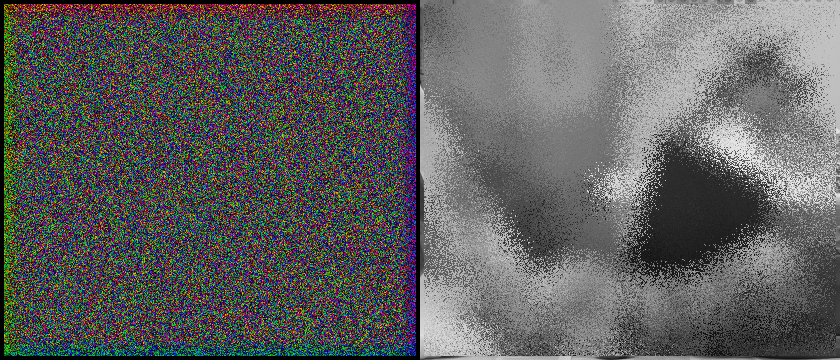
\includegraphics[width=0.8\textwidth]{images/flow-it-0.png}
  \captionof{figure}{Optical flow after initialization}
\end{minipage}

\vspace{1cm}
\begin{minipage}{0.8\textwidth}
  \centering
  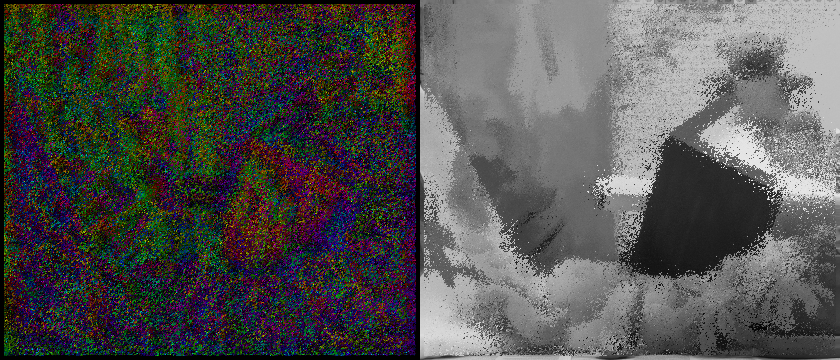
\includegraphics[width=0.8\textwidth]{images/flow-it-1.png}
  \captionof{figure}{1. iteration}
\end{minipage}

\vspace{1cm}
\begin{minipage}{0.8\textwidth}
  \centering
  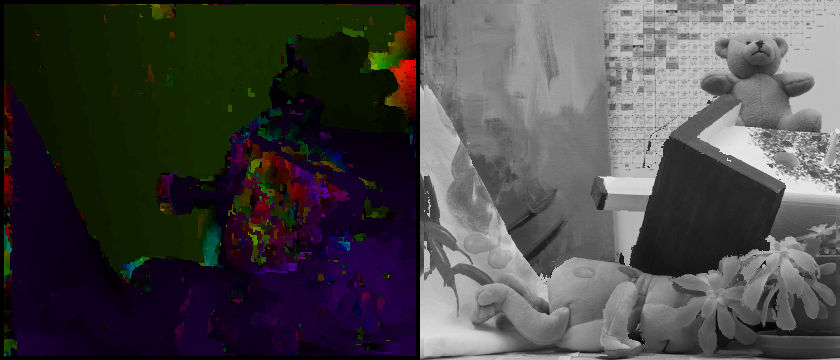
\includegraphics[width=0.8\textwidth]{images/flow-it-2.png}
  \captionof{figure}{2. iteration}
\end{minipage}

\vspace{1cm}
\begin{minipage}{0.8\textwidth}
  \centering
  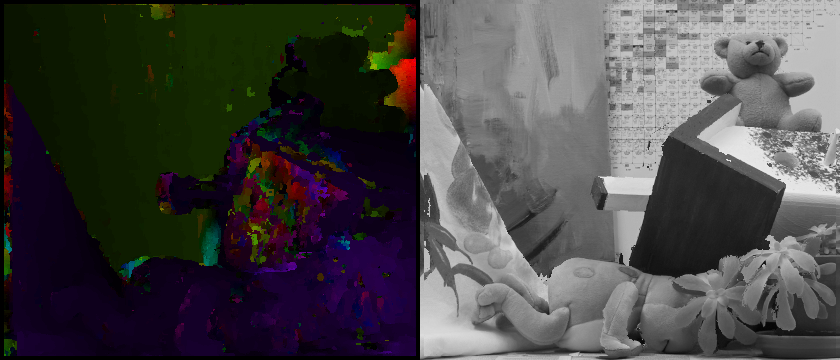
\includegraphics[width=0.8\textwidth]{images/flow-it-3.png}
  \captionof{figure}{3. iteration}
\end{minipage}

You can see that the offsets in the first iterations are more and more clustured.
The small iterations steps have a huge effect on, but the refinements in the higher
steps becomes less siginificant.


\section{Image pyramid}

\vspace{1cm}
\begin{minipage}{0.8\textwidth}
  \centering
  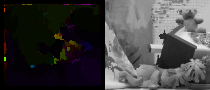
\includegraphics[width=0.5\textwidth]{images/flow-py-1-it-3.png}
  \captionof{figure}{Pyramid level 1}
\end{minipage}

\vspace{1cm}
\begin{minipage}{0.8\textwidth}
  \centering
  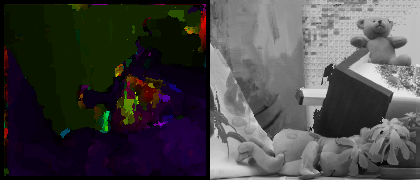
\includegraphics[width=0.65\textwidth]{images/flow-py-2-it-3.png}
  \captionof{figure}{Pyramid level 2}
\end{minipage}

\vspace{1cm}
\begin{minipage}{0.8\textwidth}
  \centering
  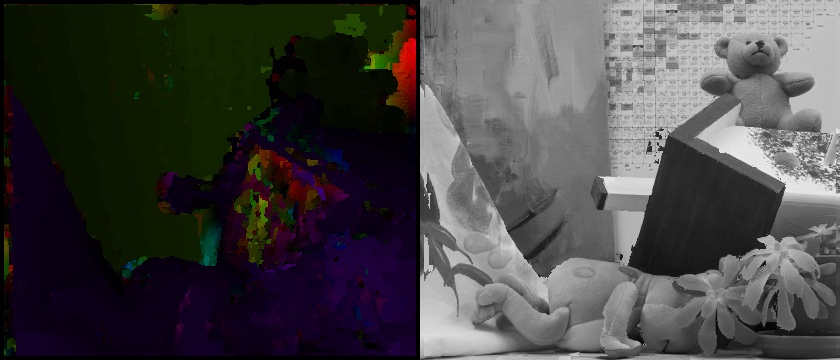
\includegraphics[width=0.8\textwidth]{images/flow-py-3-it-3.png}
  \captionof{figure}{Pyramid level 3}
\end{minipage}


\section{Other similarity meassure}

Another similarity messaure was not implemented, because the effect of this meassurements
is very small. This insight was already discovered in the Computer Vision pracical seminar
during the stereo matching task.


\section{Other similarity meassure}

There are two optical flow algorithms in the OpenCV library: the Lucas-Kanade method with pyramids and
Gunnar Farneback algorithm. The last one was already used for the first exercise. The Lucas-Kanade approach
does not compute a dense optical flow. It searches for feature points and detects their movement.


\end{document}
